\documentclass[tikz,border=16pt]{standalone}
\usepackage[T1]{fontenc}
\usepackage{lmodern}
\usetikzlibrary{positioning,arrows.meta}

\begin{document}
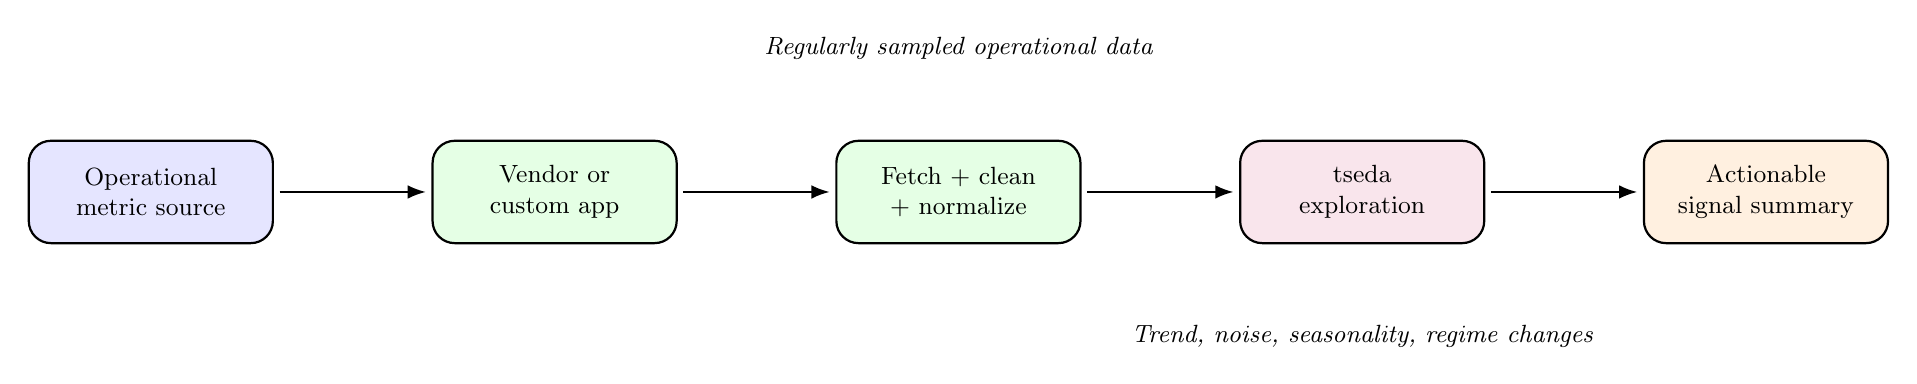
\begin{tikzpicture}[
  box/.style={draw, rounded corners=8pt, align=center, minimum width=3.1cm, minimum height=1.3cm, line width=0.8pt, font=\small},
  source/.style={box, fill=blue!10},
  platform/.style={box, fill=green!10},
  analysis/.style={box, fill=purple!10},
  action/.style={box, fill=orange!12},
  note/.style={font=\small\itshape, align=center},
  arrow/.style={-Latex, thick, shorten >=2pt, shorten <=2pt}
]

% Flow nodes
\node[source] (source1) {Operational\\metric source};
\node[platform, right=2cm of source1] (platform1) {Vendor or\\custom app};
\node[platform, right=2cm of platform1] (fetch) {Fetch + clean\\+ normalize};
\node[analysis, right=2cm of fetch] (tseda) {tseda\\exploration};
\node[action, right=2cm of tseda] (decision) {Actionable\\signal summary};

% Notes
\node[note, above=0.9cm of fetch] {Regularly sampled operational data};
\node[note, below=0.9cm of tseda] {Trend, noise, seasonality, regime changes};

% Connectors
\draw[arrow] (source1) -- (platform1);
\draw[arrow] (platform1) -- (fetch);
\draw[arrow] (fetch) -- (tseda);
\draw[arrow] (tseda) -- (decision);

\end{tikzpicture}
\end{document}
